\documentclass{beamer}

\usetheme{Warsaw}
%\usetheme{CambridgeUS}

% modification history
% created on 18 sep 2011
% modified on 25 mar

%\usepackage{amsfonts, amsmath, amssymb}

%\setbeamertemplate{theorems}[numbered]
%\setbeamertemplate{theorems}[ams style] 
\usepackage[skins,breakable]{tcolorbox}
%\usepackage[normalem]{ulem}

%\usefonttheme[onlymath]{serif}                     // change the style of math font 

%=============set slide number=================
\addtobeamertemplate{navigation symbols}{}{
    \usebeamerfont{footline}
    \usebeamercolor[fg]{footline}
    \hspace{1em}
    \insertframenumber/\inserttotalframenumber
}
\setbeamercolor{footline}{fg=black}
\setbeamerfont{footline}{series=\bfseries}


%=============set footline=====================
\setbeamertemplate{footline}
{
  \leavevmode%
  \hbox{%
  \begin{beamercolorbox}[wd=.55\paperwidth,ht=2.25ex,dp=1ex,center]{author in head/foot}%
    \usebeamerfont{author in head/foot}\insertshortauthor
  \end{beamercolorbox}%
  \begin{beamercolorbox}[wd=.45\paperwidth,ht=2.25ex,dp=1ex,center]{title in head/foot}%
    \usebeamerfont{title in head/foot}\insertshorttitle
  \end{beamercolorbox}}%
  \vskip0pt%
}

%creating a rectangle box def
\newtcbox{\mybox}[1][red]{arc=0pt,outer arc=0pt,colback=#1!10!white,colframe=#1!50!black, boxsep=0pt,left=1pt,right=1pt,top=2pt,bottom=2pt,boxrule=0pt,bottomrule=1pt,toprule=1pt}

\newtcbox{\xmybox}[1][red]{arc=7pt,colback=#1!10!white,colframe=#1!50!black,before upper={\rule[-3pt]{0pt}{10pt}},boxrule=1pt,boxsep=0pt,left=6pt,right=6pt,top=2pt,bottom=2pt}
%the ``on line'' option doesn't work. so omitting it

%===== spacing =====

\def\extraspacing{\vspace{2mm} \noindent}
\def\vgap{\vspace{2mm}}
\def\hgap{\textrm{\hspace{1mm}}}

%===== tabbing =====

\def\tab{\hspace{2mm}}
\def\tabpos{\hspace{4mm} \= \hspace{4mm} \= \hspace{4mm} \= \hspace{4mm} \=
\hspace{4mm} \= \hspace{4mm} \= \hspace{4mm} \= \hspace{4mm} \= \hspace{4mm}
\kill}
\newcommand{\mytab}[1]{\begin{tabbing}\tabpos #1\end{tabbing}}

%===== blocks =====

% \newtheorem{theorem}{Theorem}
% \newtheorem{lemma}{Lemma}
% \newtheorem{corollary}{Corollary}
% \newtheorem{proposition}{Proposition}
% \newtheorem{definition}{Definition}
% \newtheorem{problem}{Problem}

\newcommand{\cbox}[2]{\begin{tcolorbox}[arc=0mm, colframe=#1!50!black, colback=#1!10!white]#2\end{tcolorbox}}
\newcommand{\minipg}[2]{\begin{center}\begin{minipage}{#1}#2\end{minipage}\end{center}}
\newcommand{\myfrm}[1]{\begin{frame}\begin{small}#1\end{small}\end{frame}} 
\newcommand{\myitems}[1]{\begin{itemize}#1\end{itemize}}
\newcommand{\myenums}[1]{\begin{enumerate}#1\end{enumerate}}
\newcommand{\myfig}[1]{\begin{figure}\centering #1\end{figure}}
    
%===== math macros =====
\newcommand{\bm}[1]{\textrm{\boldmath${#1}$}}
%\newcommand{\smat}[2]{\left[\begin{tabular}{#1}#2\end{tabular}\right]}
%\newcommand{\bmat}[2]{\left|\begin{tabular}{#1}#2\end{tabular}\right|}
\newcommand{\bmat}[1]{\begin{bmatrix}#1\end{bmatrix}}
\newcommand{\vmat}[1]{\begin{vmatrix}#1\end{vmatrix}}
\newcommand{\myeqn}[1]{\begin{eqnarray}#1\end{eqnarray}}
\newcommand{\set}[1]{\{#1\}}

\def\eps{\epsilon}
\def\fr{\frac}
\def\lc{\lceil}
\def\lf{\lfloor}
\def\rc{\rceil}
\def\rf{\rfloor}
\def\Pr{\textrm{\boldmath$Pr$}}
\def\expt{\textrm{\boldmath$E$}}
\def\real{\mathbb{R}}
\def\int{\mathbb{Z}}
\def\*{\star}
\def\tO{\tilde{O}}

\DeclareMathOperator*{\argmin}{arg\,min}
\DeclareMathOperator*{\polylg}{polylg}
\DeclareMathOperator*{\polylog}{polylog}
\DeclareMathOperator*{\intr}{\cap}

\def\nn{\nonumber}
\def\mit{\mathit}


%===== misc =====

\def\done{\hspace*{\fill} $\framebox[2mm]{}$}	% end of proof
\def\ttt{\texttt}

%===== coloring =====
\newcommand{\red}[1]{\textcolor{red}{#1}}
\newcommand{\bred}[1]{\textcolor{red}{\bf #1}}
\newcommand{\blue}[1]{\textcolor{blue}{\bf #1}}

\usepackage{color}
\usepackage{graphicx}
\usepackage{multirow}
\usepackage{wrapfig}
\usepackage[skins,breakable]{tcolorbox}

\def\done{\hfill$\square$}
\def\ttt{\texttt}
\def\vgap{\vspace{5mm}}

\title[DATABASE SYSTEM PRINCIPLES]{Query Processing 2:\\ I/O-Efficient Sorting}

\author[Yufei Tao @ NTU]{Yufei Tao}
\institute[]{}
\date{}

% \def\dtm{\mathit{d\mbox{-}tm}}
% \def\ftm{\mathit{f\mbox{-}tm}}
\def\bestext{\mathit{best\mbox{-}ext}}

\begin{document}
%-------------------------------------------------------------
\begin{frame}
    \titlepage
%     \begin{tcolorbox}[arc=0mm, colframe=green!50!black, colback=green!10!white] 
%     \end{tcolorbox}
\end{frame}
%-------------------------------------------------------------
\begin{frame}
\begin{small}
    %Sorting is a fundamental operation in database systems.
    This lecture will introduce an algorithm for sorting \bred{disk-resident} data
    with a small \bred{I/O cost}.

    %\vgap
\end{small}    
\end{frame}
%-------------------------------------------------------------
\myfrm{
    \xmybox{(Disk-Based) Sorting}

    \vgap

    $\red{R}$: a set of elements drawn from a total order, each represented with the same number of words. \\
    $\red{B} =$ the number of disk blocks that $R$ occupies. \\
    $\red{M} =$ the number of memory blocks (a.k.a., the buffer blocks). \\

    \vgap

    \blue{Goal:} Produce a sorted list of the elements in $R$ on disk.

    \vgap

    \cbox{blue}{
        \blue{Think:} Why not use a ``memory-sorting'' algorithm such as merge sort or quick sort?
    }
}
%-------------------------------------------------------------
\myfrm{
    \cbox{yellow}{
        Next, we will take a ``detour'' to discuss a stand-alone problem called \bred{merging}. As we will see, a fast algorithm for merging implies a fast algorithm for sorting.
    }
}
%-------------------------------------------------------------
\myfrm{
    \xmybox{(Disk-Based) Merging}

    \vgap

    $\red{M} =$ the number of memory blocks (a.k.a., the buffer blocks). \\
    We have $\red{R_1}, \red{R_2}, ..., \red{R_{M-1}}$ where
    \myitems{
        \item all the elements in $R_1, ..., R_{M-1}$ are drawn from a total order, each represented with the same number of words;
        \item $R_1, ..., R_{M-1}$ are mutually disjoint;
        \item each $R_i$ ($1 \le i \le M-1$) is \bred{sorted}.
    }
    For each $\red{i} \in [1, M-1]$, denote by $\red{B_i}$ the number of disk blocks that $R_i$ occupies.

    \vgap

    \blue{Goal:} Produce a sorted list of $R_1 \cup R_2 \cup ... \cup R_{M-1}$ on disk.
}
%-------------------------------------------------------------
\myfrm{
    \xmybox{(Disk-Based) Merging}

    \vgap

    \blue{Example:} $M = 5$.
    \begin{center}
        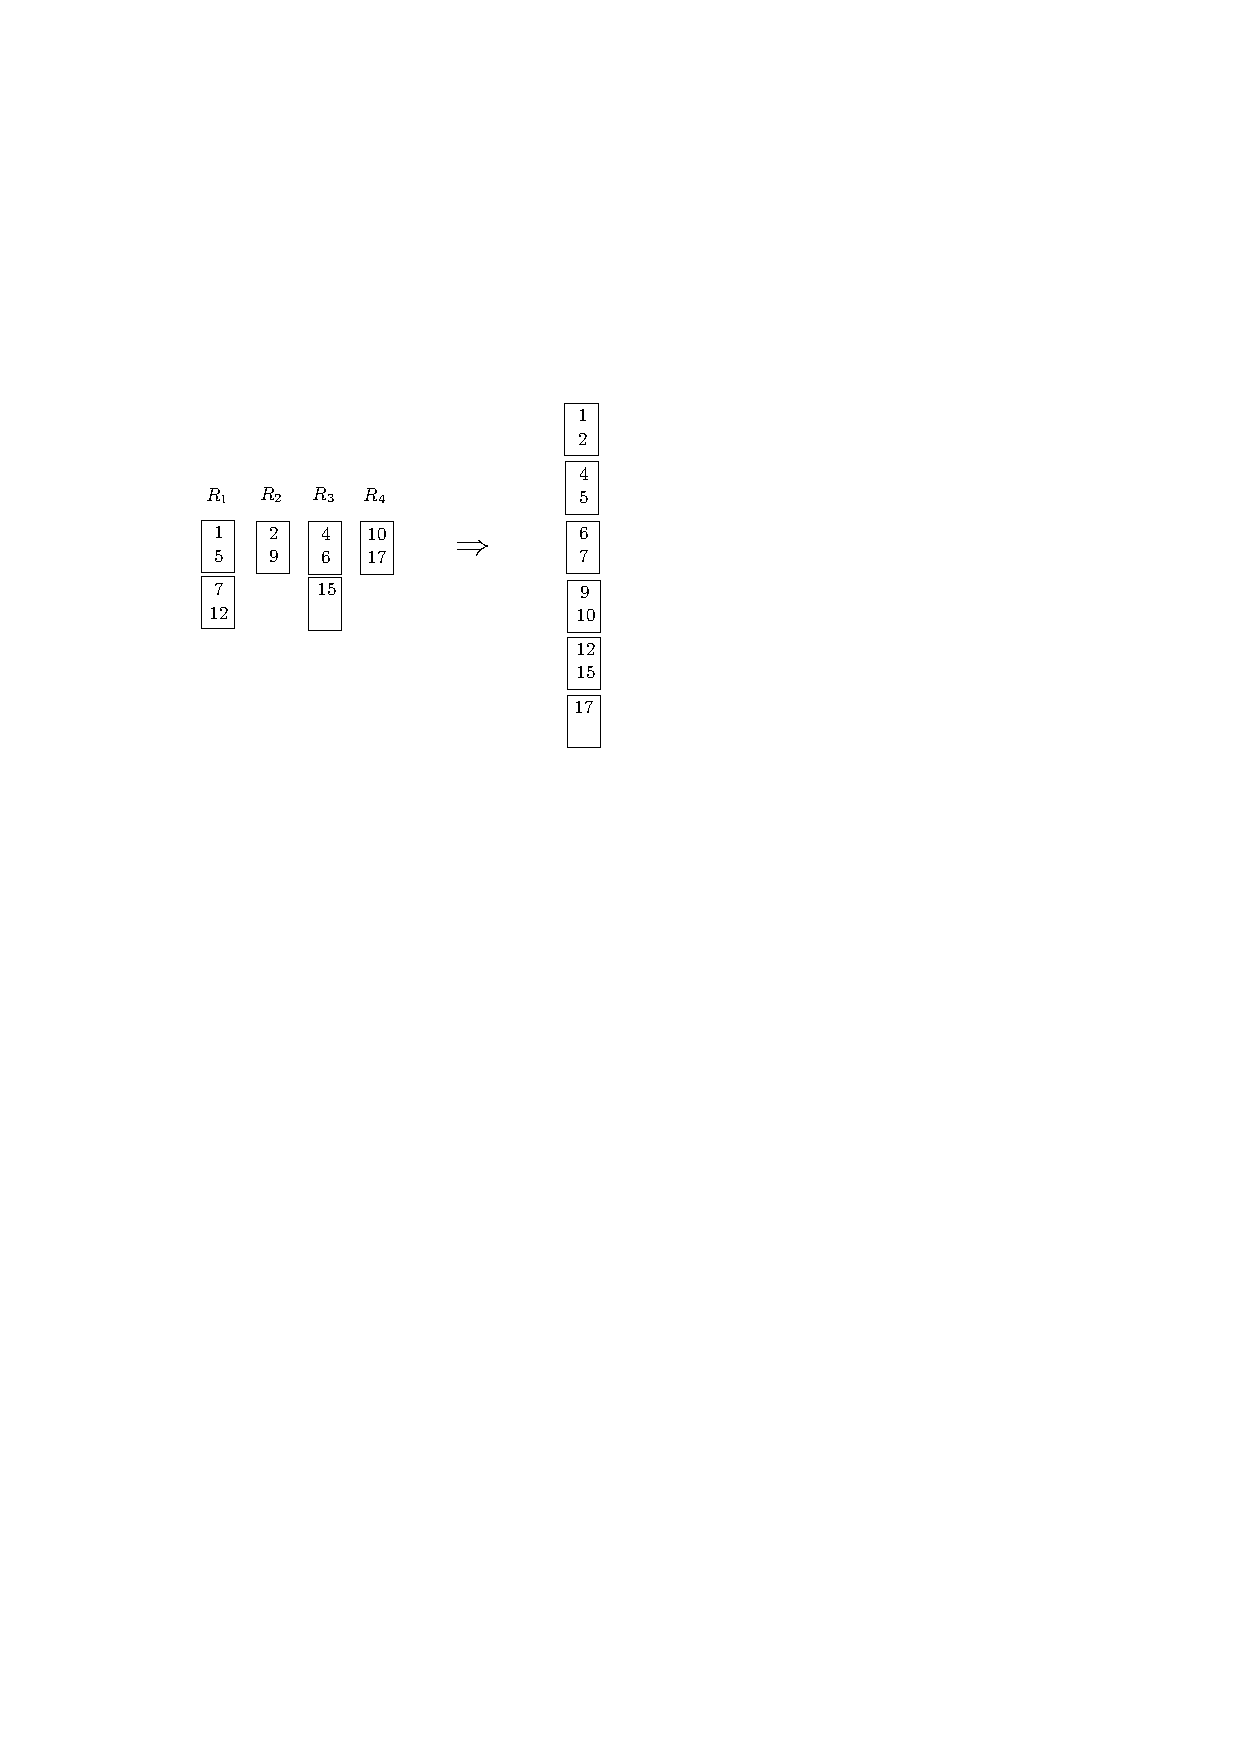
\includegraphics[height=40mm]{./artwork/em-merge0}
    \end{center}

}
%-------------------------------------------------------------
\myfrm{
    \xmybox{(Disk-Based) Merging}

    \vgap

    To solve the problem, we allocate one memory block to each $R_i$ ($1 \le i \le M-1$) as its \blue{input buffer}. This consumes $M - 1$ memory blocks. The remaining memory block is allocated as the \blue{output buffer}.

    \vgap

    Load the first page of each $R_i$ ($1 \le i \le M-1$) into its input buffer.

    \begin{center}
        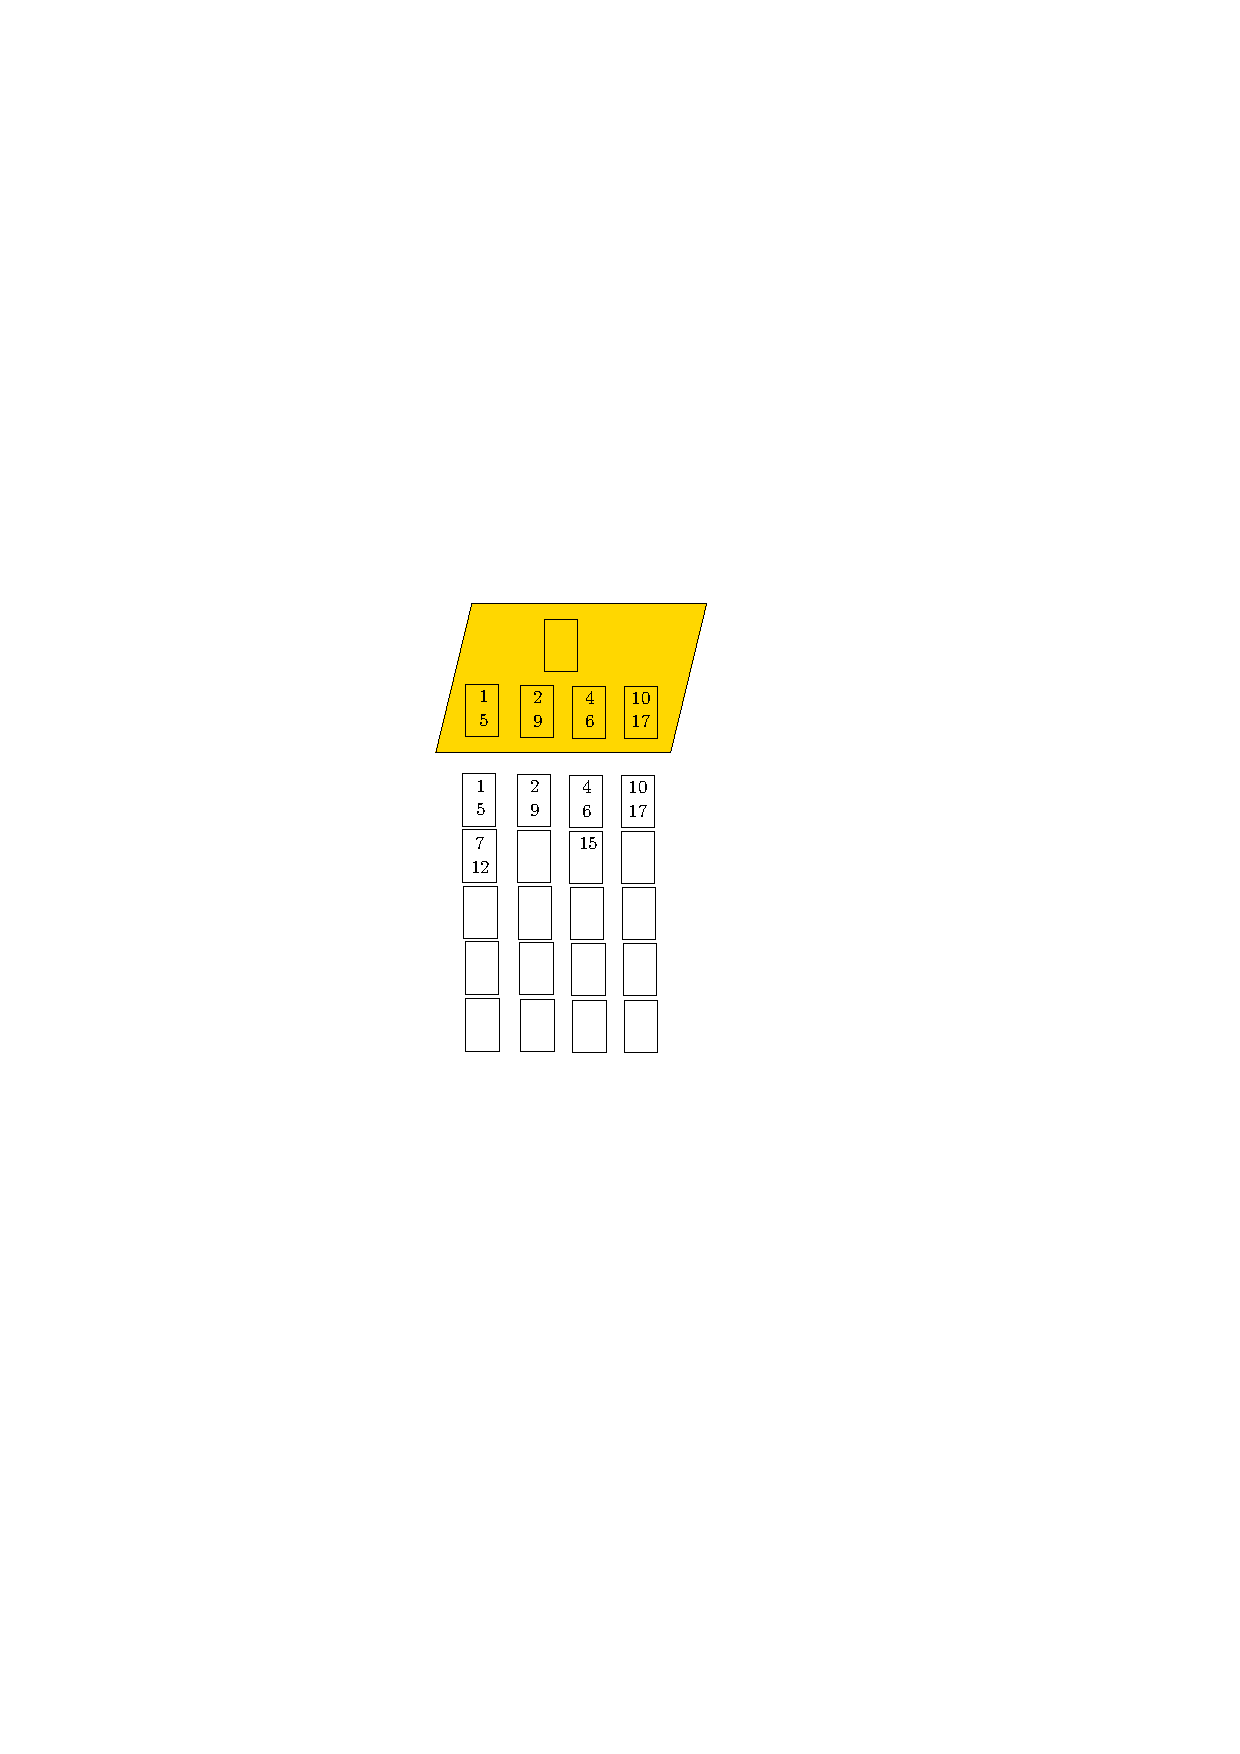
\includegraphics[height=40mm]{./artwork/em-merge1}
    \end{center}

}
%-------------------------------------------------------------
\myfrm{
    \xmybox{(Disk-Based) Merging}

    \vgap

    Move the smallest integer in the input buffers to the output buffer \bred{until}
    \myitems{
        \item \bred{either} the output buffer is full
        \item \bred{or} an input buffer becomes empty.
    }

    \begin{center}
        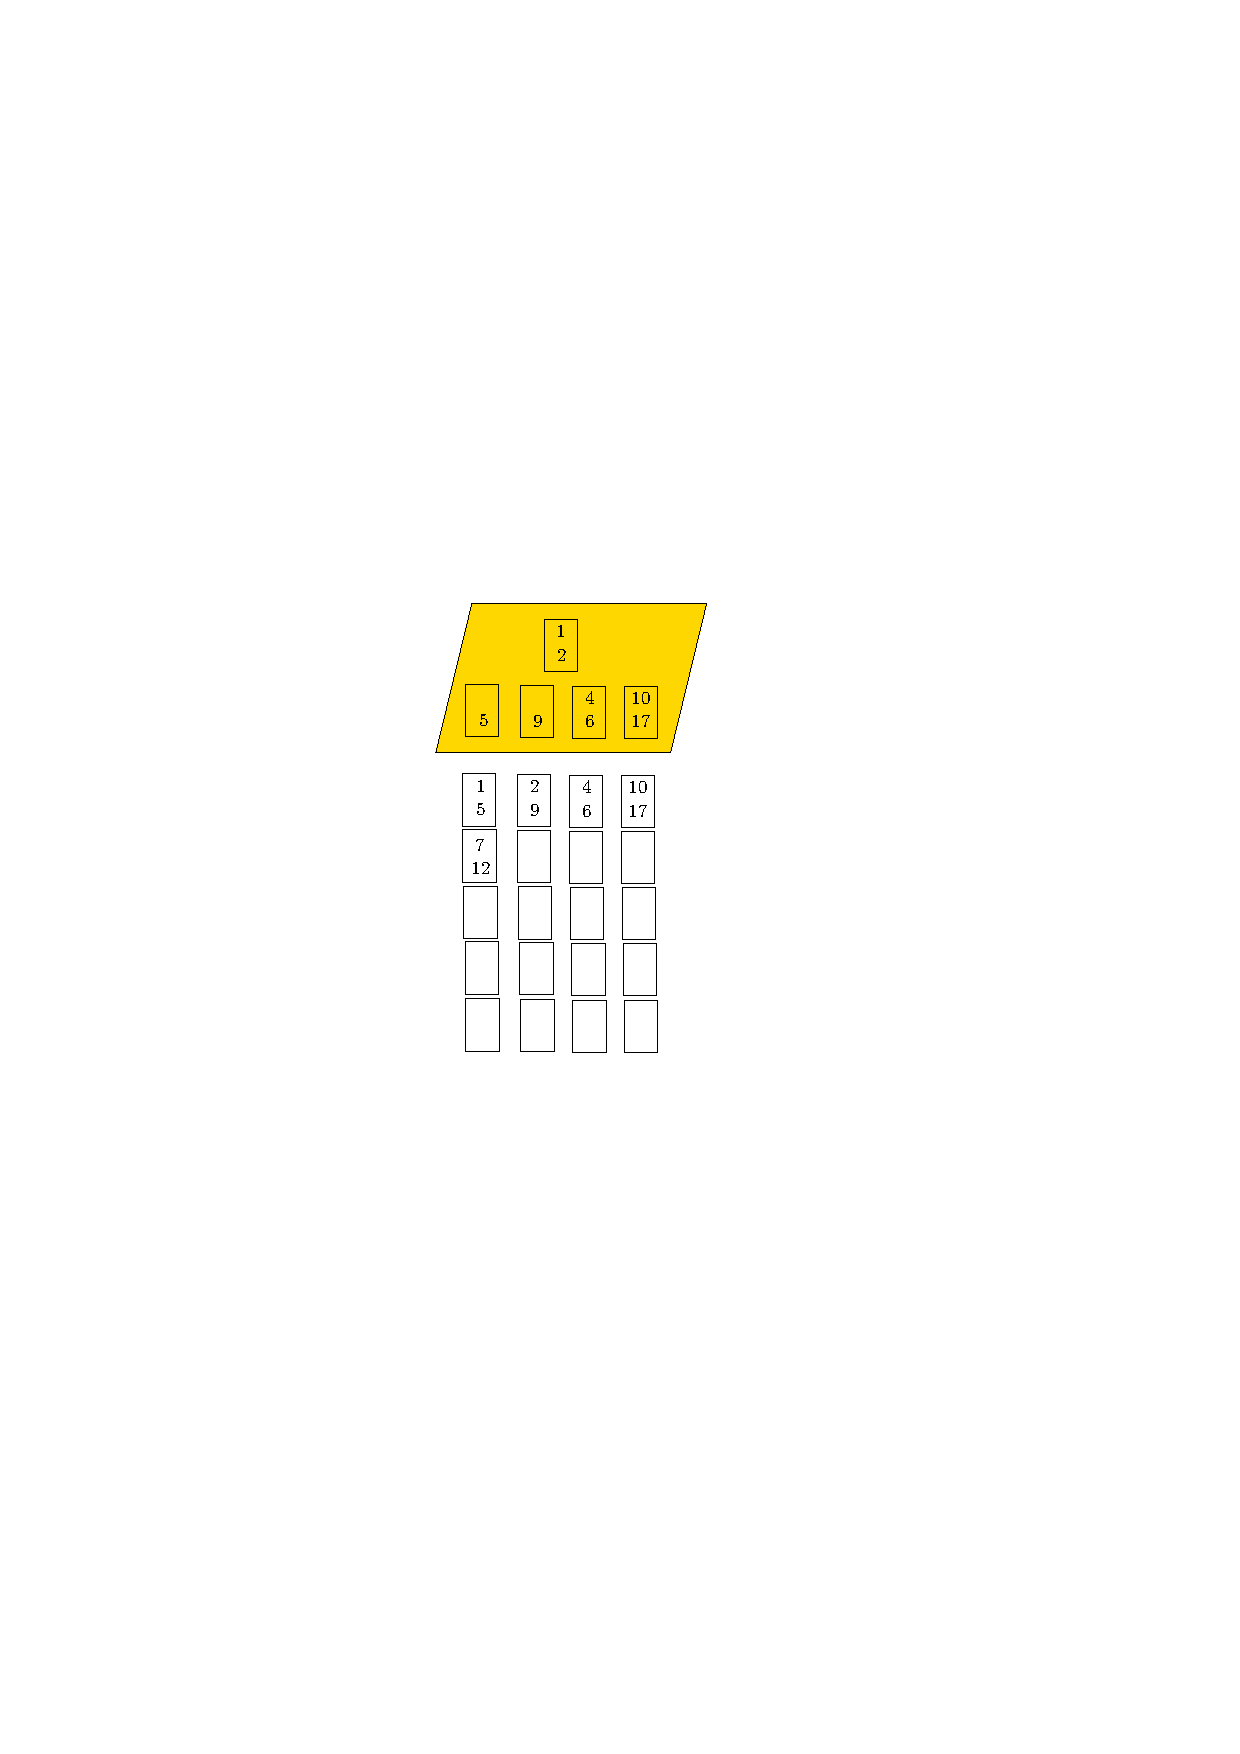
\includegraphics[height=40mm]{./artwork/em-merge2}
    \end{center}

}
%-------------------------------------------------------------
\myfrm{
    \xmybox{(Disk-Based) Merging}

    \vgap

    If the output buffer is full, output it to the sorted file on disk.

    \begin{center}
        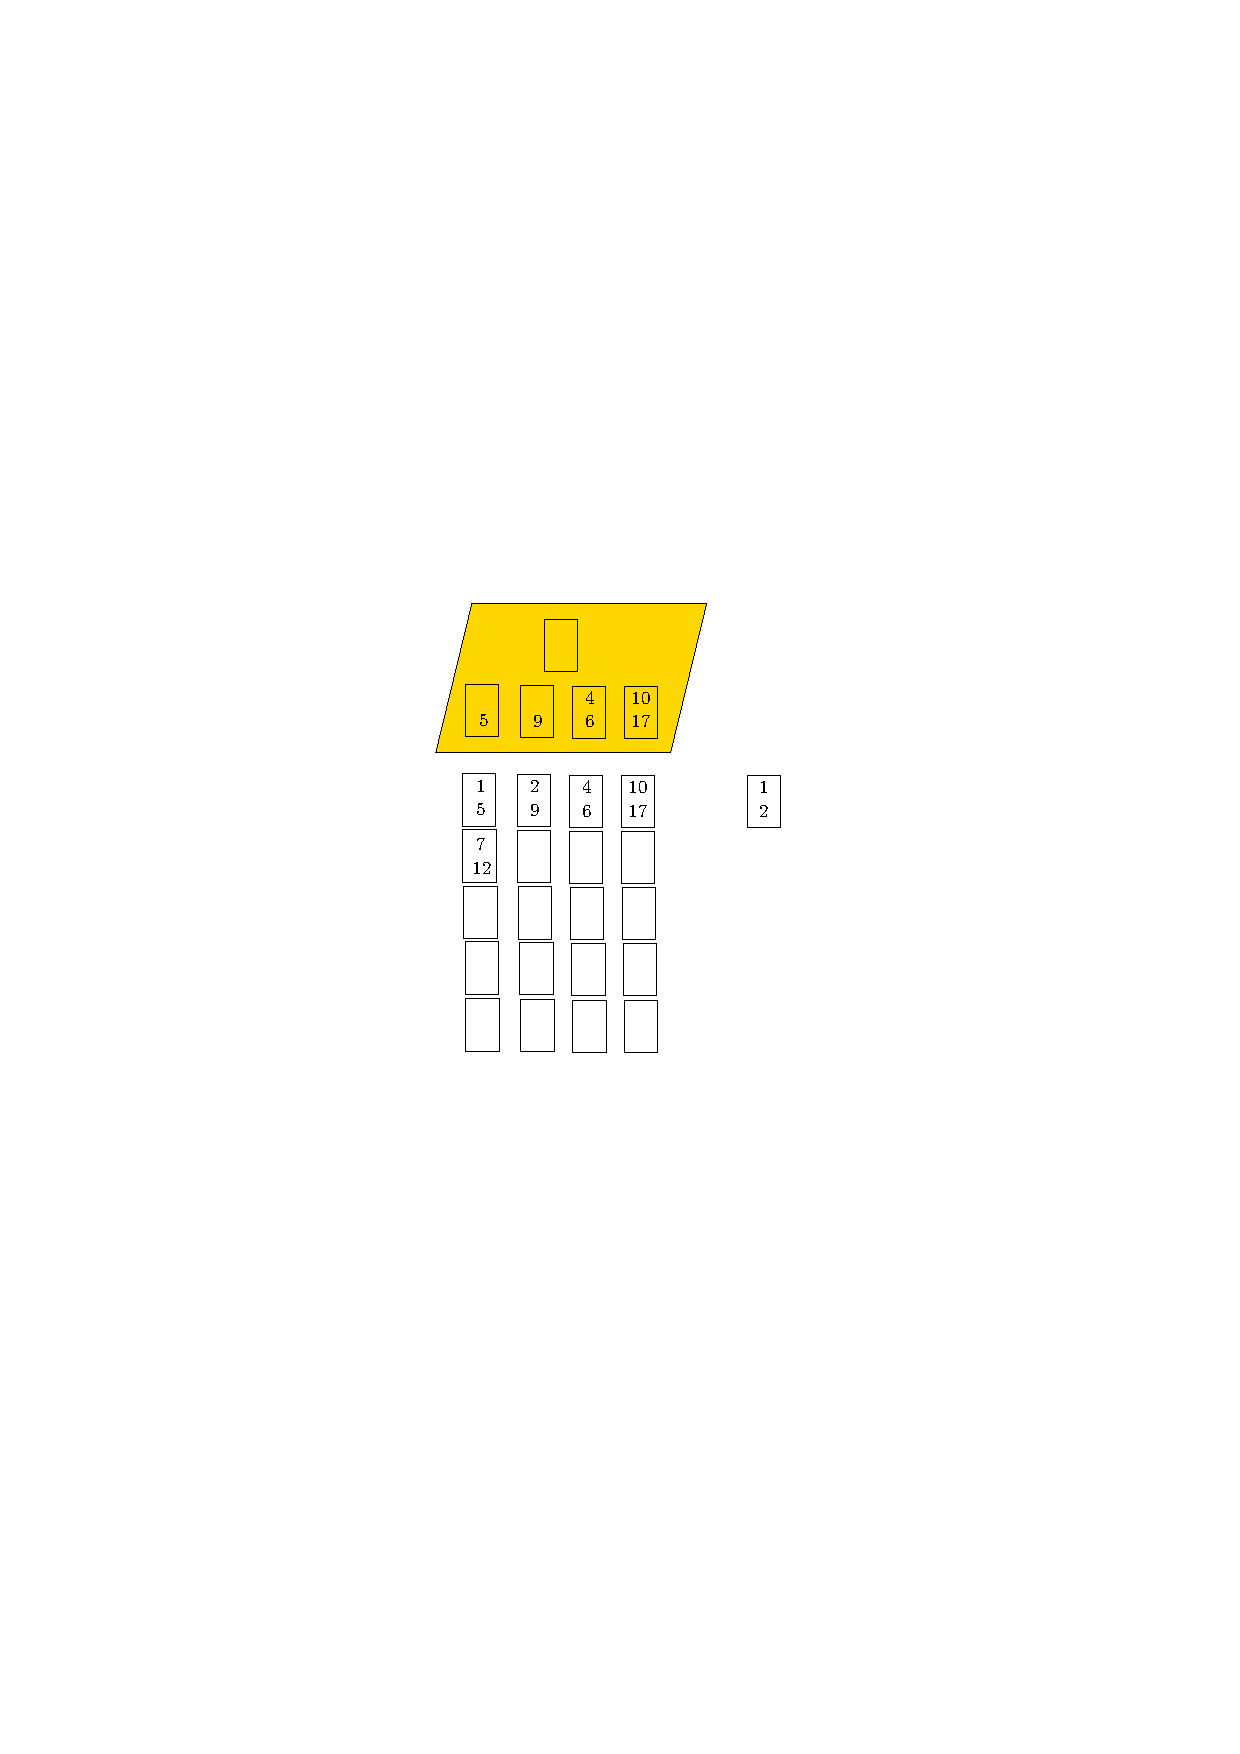
\includegraphics[height=40mm]{./artwork/em-merge3}
    \end{center}

}
%-------------------------------------------------------------
\myfrm{
    \xmybox{(Disk-Based) Merging}

    \vgap

    Move the smallest integer in the input buffers to the output buffer \bred{until}
    \myitems{
        \item \bred{either} the output buffer is full
        \item \bred{or} an input buffer becomes empty.
    }

    \begin{center}
        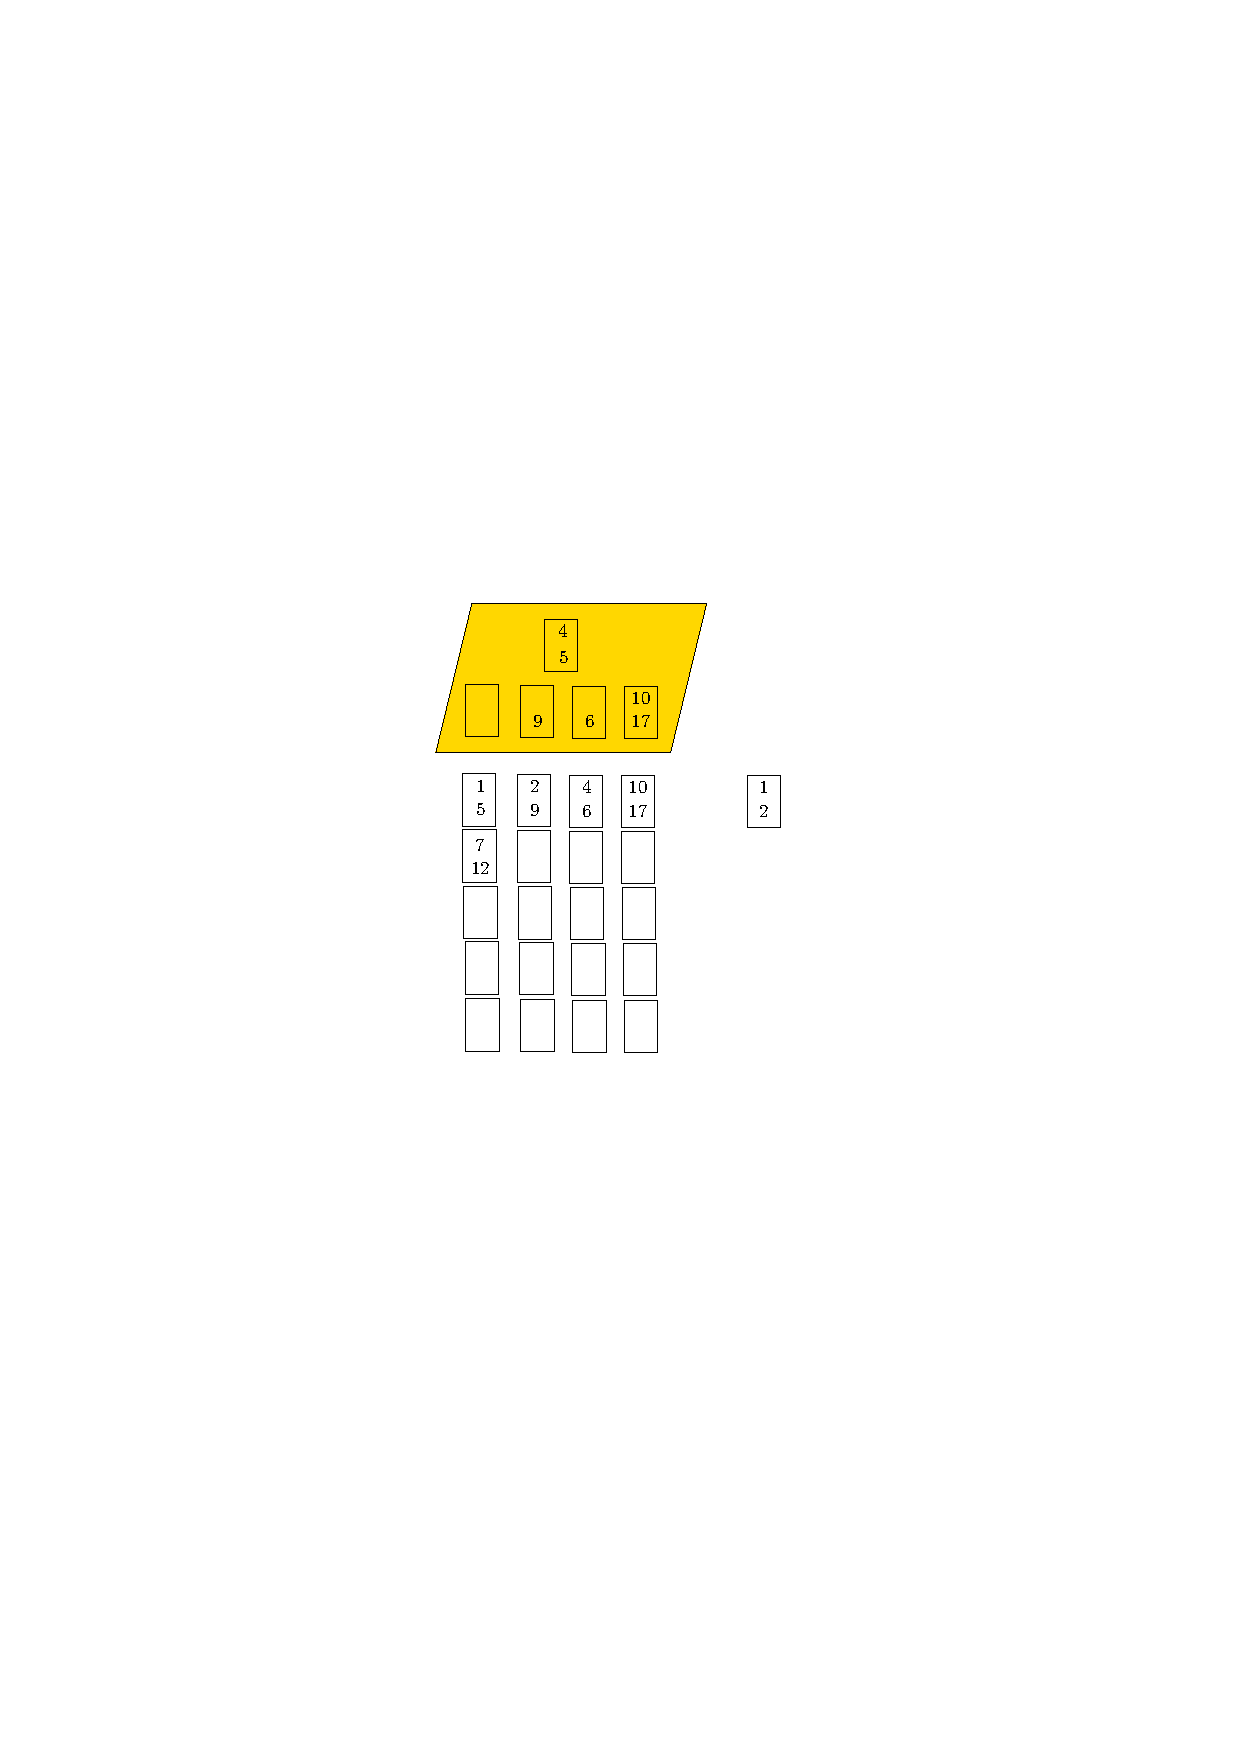
\includegraphics[height=40mm]{./artwork/em-merge4}
    \end{center}

}
%-------------------------------------------------------------
\myfrm{
    \xmybox{(Disk-Based) Merging}

    \vgap

    If the output buffer is full, output it to the sorted file on disk.

    \begin{center}
        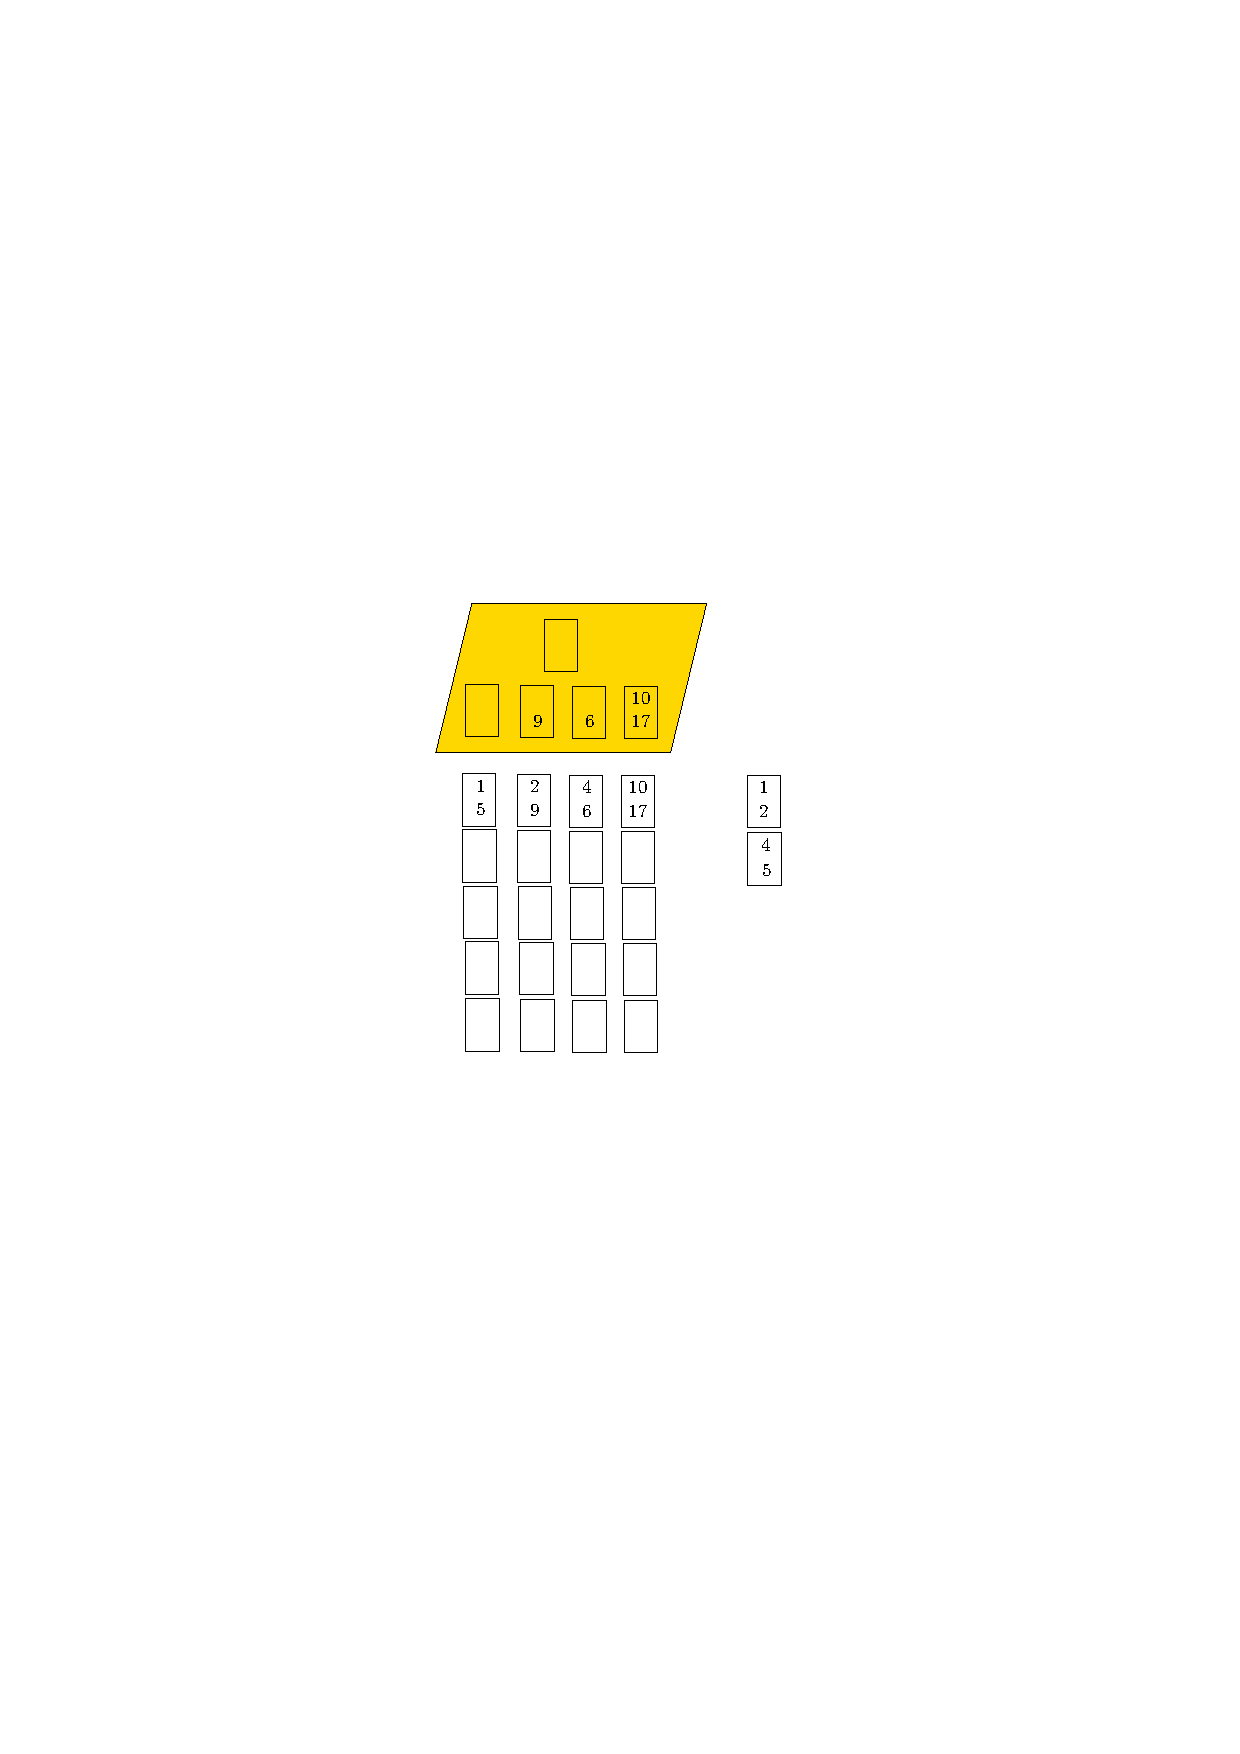
\includegraphics[height=40mm]{./artwork/em-merge5}
    \end{center}

}
%-------------------------------------------------------------
\myfrm{
    \xmybox{(Disk-Based) Merging}

    \vgap

    Move the smallest integer in the input buffers to the output buffer \bred{until}
    \myitems{
        \item \bred{either} the output buffer is full
        \item \bred{or} an input buffer becomes empty.
    }
    If an input buffer is empty --- say the buffer is for $\red{R_i}$ --- fill it with the next block of $R_i$ (if it exists).

    \begin{center}
        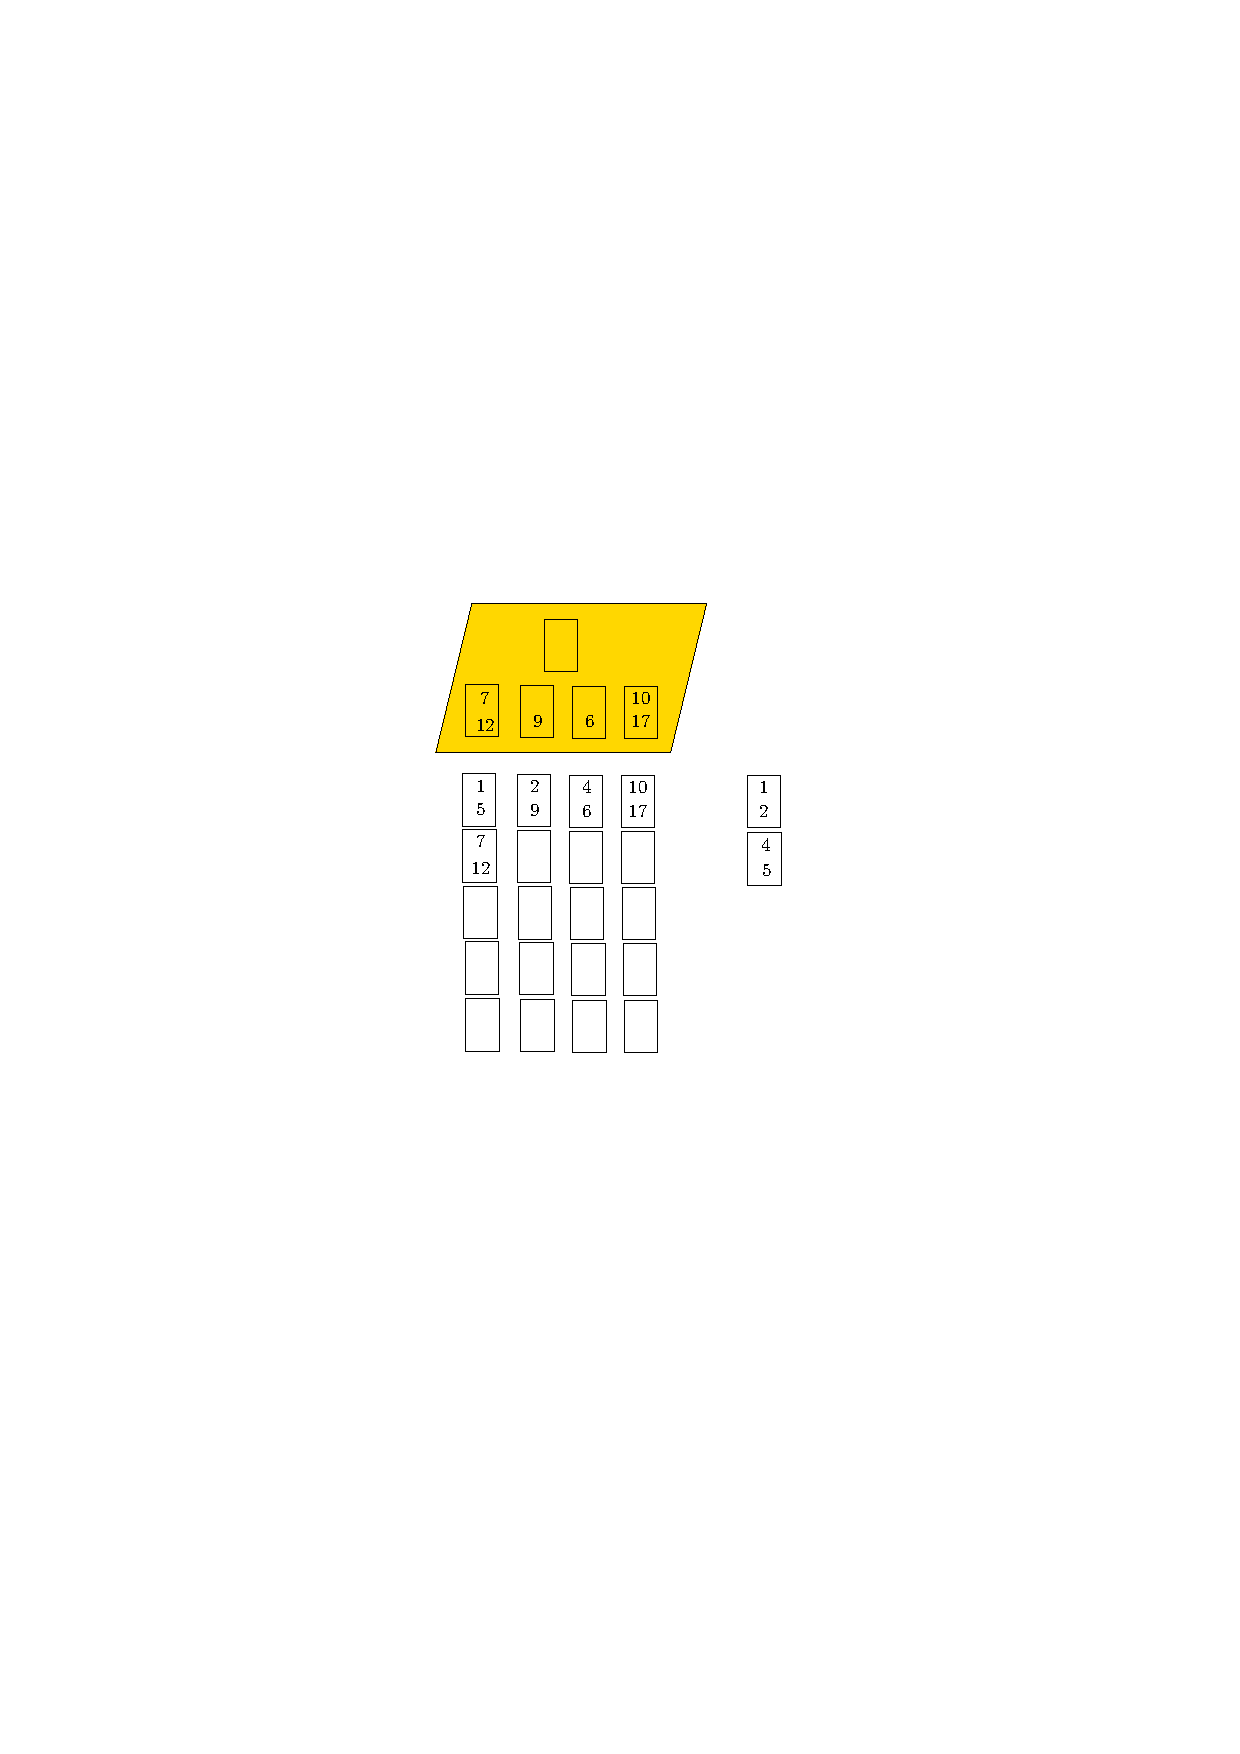
\includegraphics[height=40mm]{./artwork/em-merge6}
    \end{center}

}
%-------------------------------------------------------------
\myfrm{
    \xmybox{(Disk-Based) Merging}

    \vgap

    Repeat the above steps until all of $R_1, ..., R_{M-1}$ have been exhausted.

    \begin{center}
        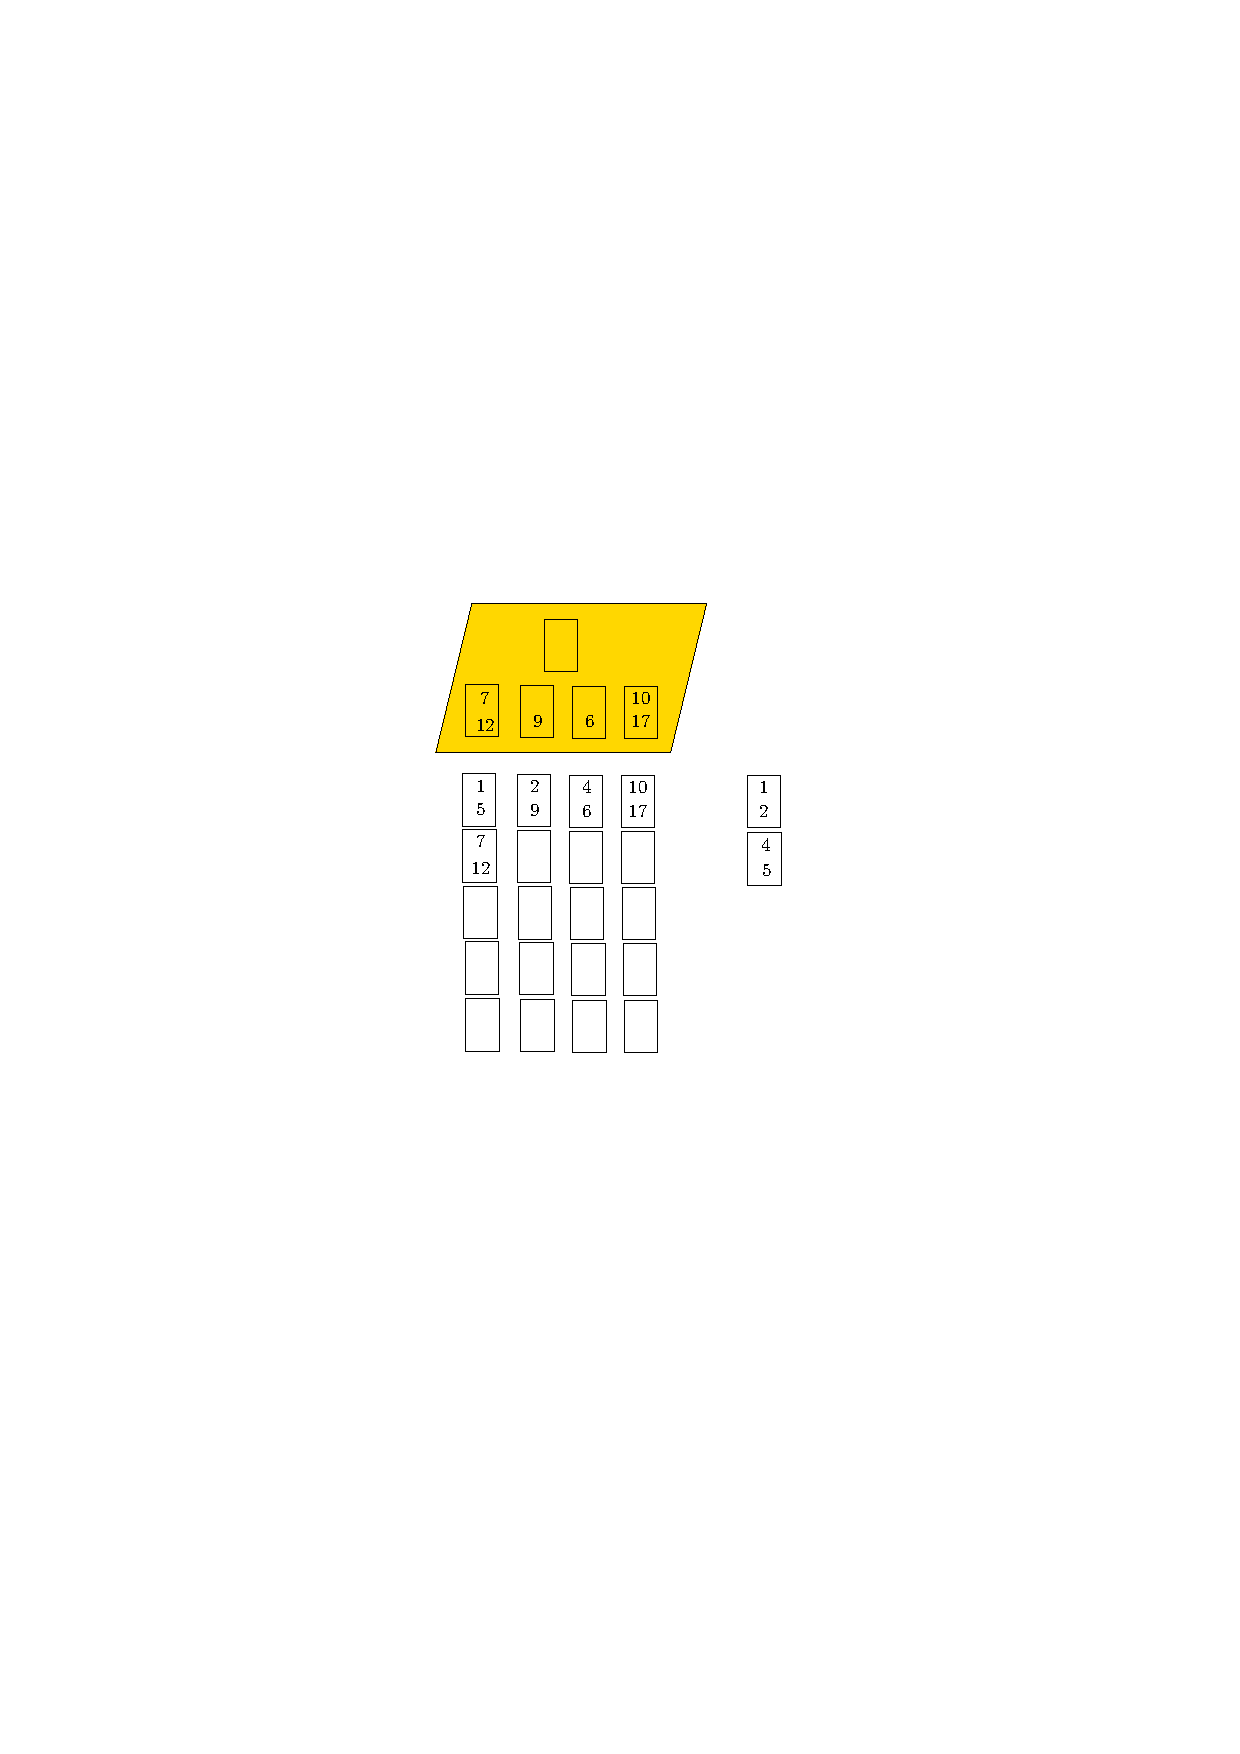
\includegraphics[height=40mm]{./artwork/em-merge6}
    \end{center}

}
%-------------------------------------------------------------
\myfrm{
    \xmybox{(Disk-Based) Merging}

    \vgap

    I/O cost:
    \myitems{
        \item Number of Read I/Os $= \sum_{i=1}^{M-1} B_i$\\
        (every input block read once)
        \item Number of Write I/Os $\le \sum_{i=1}^{M-1} B_i$ \\
        (the sorted file cannot have more blocks).
    }

    \cbox{green}{
        Total I/O cost $\le 2 \sum_{i=1}^{M-1} B_i$.
    }
}
%-------------------------------------------------------------
\myfrm{
    \cbox{yellow}{
        \centering
        We now return to the sorting problem.
    }
}
%-------------------------------------------------------------
\myfrm{
    \xmybox{(Disk-Based) Sorting}

    Recall that the input is $\red{R}$, which occupies $\red{B}$ blocks.

    \vgap


    \mybox[green]{The Initial Step}

    Chop $R$ into $\red{n_0} = \red{\lc {B/M} \rc}$ \blue{runs}, each consisting of $M$ consecutive blocks (except possibly the last run).

    \vgap

    \bred{For each run}: load its elements into memory, sort them, and write them back to the disk, replacing the original run --- this produces a \blue{sorted run}.

    \begin{center}
        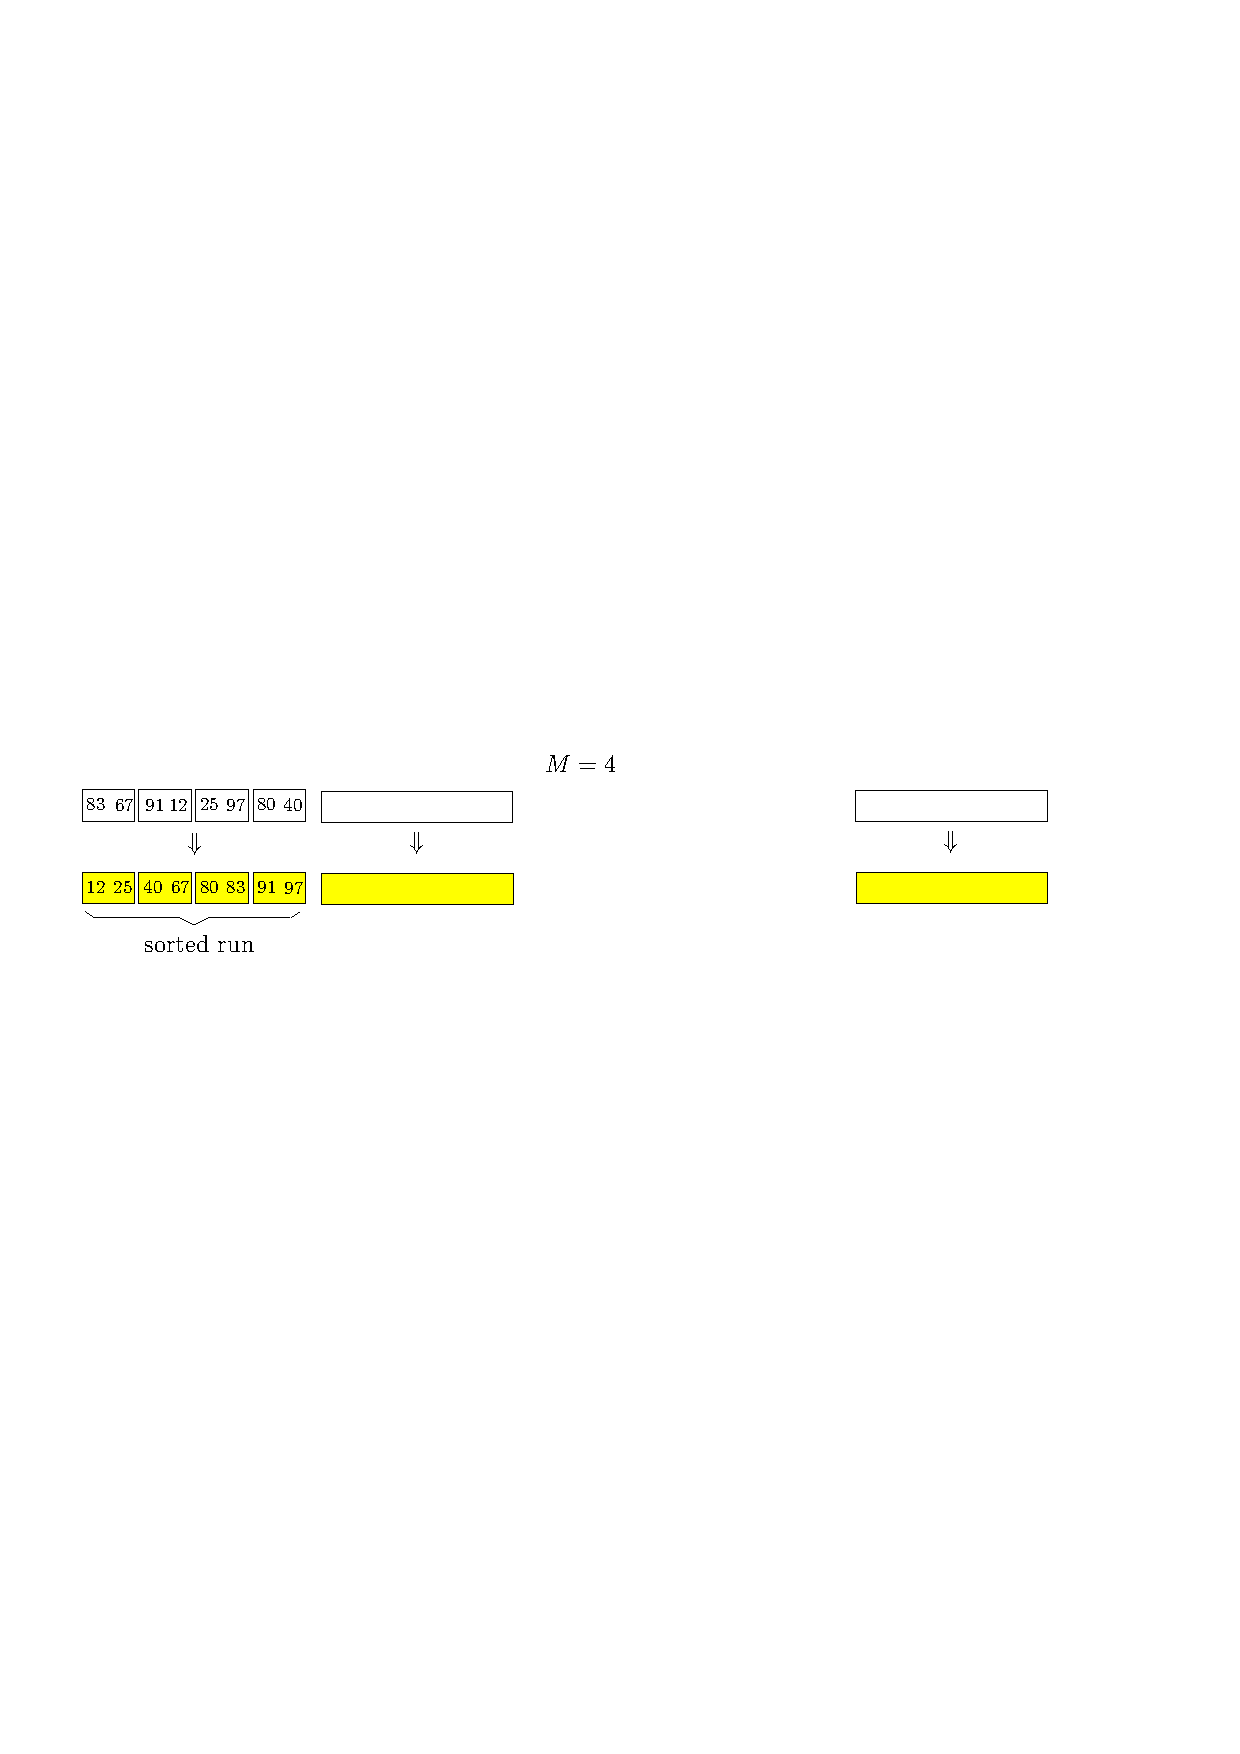
\includegraphics[height=20mm]{./artwork/em-sort0}
    \end{center}

    I/O cost = $2 \cdot B$ (\blue{think:} why 2?)
}
%-------------------------------------------------------------
\myfrm{
    \xmybox{(Disk-Based) Sorting}

    \mybox[green]{Merging Step 1}

    \bred{For every $M - 1$ sorted runs}: merge them into one sorted run. \\

    The number of new sorted runs is
    \myeqn{
        \red{n_1} = \lc n_0 / (M-1) \rc. \nn
    }
    A new sorted run has $M (M-1)$ blocks (except possibly for the last one).


    %\vgap

    \begin{center}
        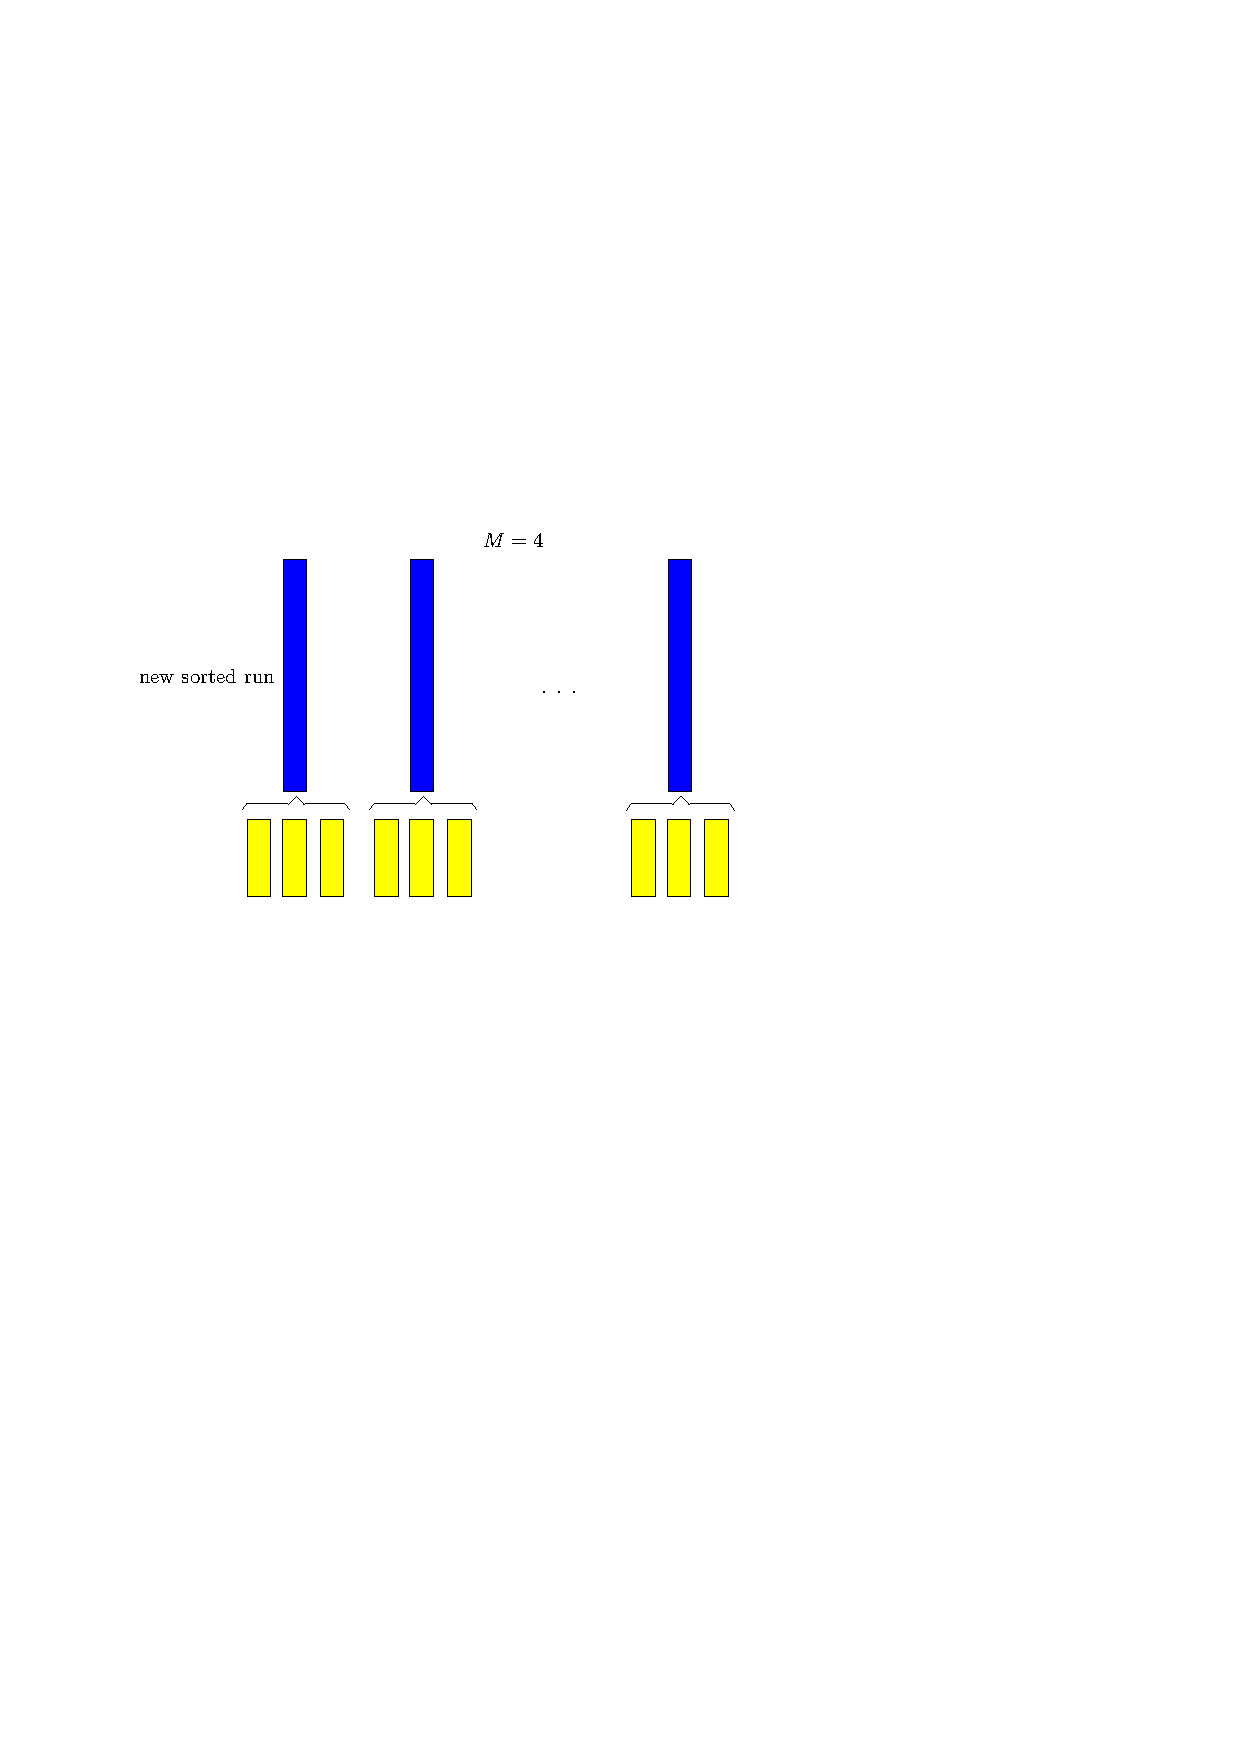
\includegraphics[height=35mm]{./artwork/em-sort1}
    \end{center}

    I/O cost $\le 2 \cdot B$ (\blue{think:} why?)
}
%-------------------------------------------------------------
\myfrm{
    \xmybox{(Disk-Based) Sorting}

    \mybox[green]{Merging Step $\red{i} \ge 1$}

    \bred{For every $M - 1$ sorted runs from the last step}: merge them into one sorted run.
    The number of new sorted runs is
    \myeqn{
        \red{n_i} = \lc n_{i-1} / (M-1) \rc. \nn
    }
    A new sorted run has $M (M-1)^i$ blocks (except possibly for the last one).


    \vgap

    I/O cost $\le 2 \cdot B$.

    \vgap

    When $n_i = 1$, we are done.
}
%-------------------------------------------------------------
\myfrm{
    \xmybox{(Disk-Based) Sorting}

    \vgap

    $\red{h} =$ the total number of merging steps.

    \cbox{blue}{
        The total I/O cost of sorting is at most $
            2 \cdot B \cdot (h + 1).
        $
    }

    \vgap

    \blue{Remark:} In practice, we typically have $B \le M(M-1)$, in which case there is only one merging step and the I/O cost is $4 B$.
}
%-------------------------------------------------------------
\end{document} 
